\pdfminorversion=4
\documentclass[aspectratio=169]{beamer}

\mode<presentation>
{
  \usetheme{default}
  \usecolortheme{default}
  \usefonttheme{default}
  \setbeamertemplate{navigation symbols}{}
  \setbeamertemplate{caption}[numbered]
  \setbeamertemplate{footline}[frame number]  % or "page number"
  \setbeamercolor{frametitle}{fg=white}
  \setbeamercolor{footline}{fg=black}
} 

\usepackage[english]{babel}
\usepackage[utf8x]{inputenc}
\usepackage{tikz}
\usepackage{courier}
\usepackage{array}
\usepackage{bold-extra}
\usepackage{minted}
\usepackage[thicklines]{cancel}
\usepackage{fancyvrb}

\xdefinecolor{dianablue}{rgb}{0.18,0.24,0.31}
\xdefinecolor{darkblue}{rgb}{0.1,0.1,0.7}
\xdefinecolor{darkgreen}{rgb}{0,0.5,0}
\xdefinecolor{darkgrey}{rgb}{0.35,0.35,0.35}
\xdefinecolor{darkorange}{rgb}{0.8,0.5,0}
\xdefinecolor{darkred}{rgb}{0.7,0,0}
\definecolor{darkgreen}{rgb}{0,0.6,0}
\definecolor{mauve}{rgb}{0.58,0,0.82}

\title[2019-10-03-yana-david]{Conversation with Yana and David about Awkward 1.0}
\author{Jim Pivarski}
\institute{Princeton University -- IRIS-HEP}
\date{October 3, 2019}

\usetikzlibrary{shapes.callouts}

\begin{document}

\logo{\pgfputat{\pgfxy(0.11, 7.4)}{\pgfbox[right,base]{\tikz{\filldraw[fill=dianablue, draw=none] (0 cm, 0 cm) rectangle (50 cm, 1 cm);}\mbox{\hspace{-8 cm}
\includegraphics[height=1 cm]{princeton-logo-long.png}\hspace{0.1 cm}\raisebox{0.1 cm}{
\includegraphics[height=0.8 cm]{iris-hep-logo-long.png}}\hspace{0.1 cm}}}}}

\begin{frame}
  \titlepage
\end{frame}

\logo{\pgfputat{\pgfxy(0.11, 7.4)}{\pgfbox[right,base]{\tikz{\filldraw[fill=dianablue, draw=none] (0 cm, 0 cm) rectangle (50 cm, 1 cm);}\mbox{\hspace{-8 cm}
\includegraphics[height=1 cm]{princeton-logo.png}\hspace{0.1 cm}\raisebox{0.1 cm}{
\includegraphics[height=0.8 cm]{iris-hep-logo.png}}\hspace{0.1 cm}}}}}

% Uncomment these lines for an automatically generated outline.
%\begin{frame}{Outline}
%  \tableofcontents
%\end{frame}

% START START START START START START START START START START START START START

\begin{frame}{Context: columnar data analysis}
\large
\vspace{0.5 cm}
\begin{columns}
\column{1.1\linewidth}
\begin{itemize}\setlength{\itemsep}{1 cm}
\item \textcolor{darkblue}{\Large uproot}: reads columnar data (``split'' in ROOT terminology) from ROOT files without reconstructing objects---leaving them as arrays or jagged arrays.

\vspace{0.25 cm}
\textcolor{gray}{\normalsize (used by CMS, ATLAS, LHCb, NOvA, nuclear physics, theory, and gamma-ray astronomy)}

\item \textcolor{darkblue}{\Large awkward-array}: presents columnar data as though they were arrays of objects.

\vspace{0.25 cm}
\textcolor{gray}{\normalsize (used by 41 other projects on GitHub, including uproot and Coffea)}

\item \textcolor{darkblue}{\Large Coffea}: more fully featured data analysis package, developed by Fermilab physicists.

\vspace{0.25 cm}
\textcolor{gray}{\normalsize (used by at least 8 CMS analyses)}
\end{itemize}
\end{columns}
\end{frame}

\begin{frame}{Columnar data structures}
\vspace{0.2 cm}
\begin{center}
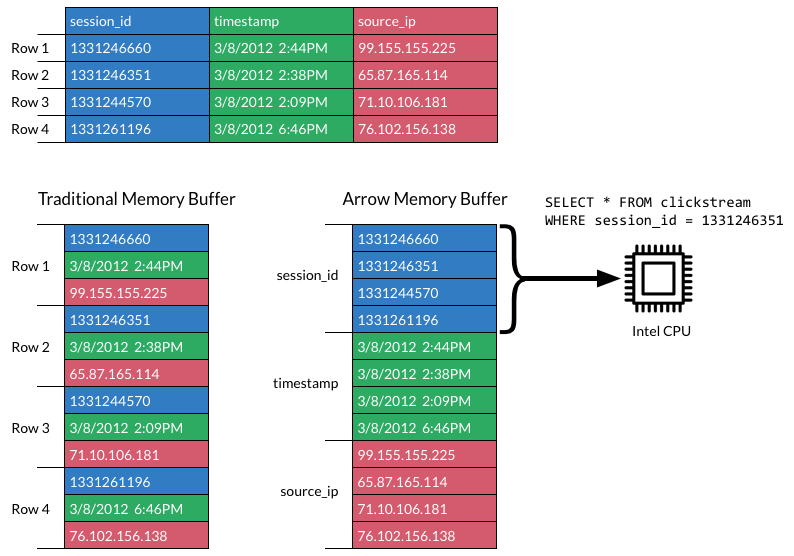
\includegraphics[width=0.7\linewidth]{simd.png}
\end{center}

Source: \textcolor{blue}{\url{http://arrow.apache.org}}
\end{frame}

\begin{frame}{Columnar data structures}
\begin{center}
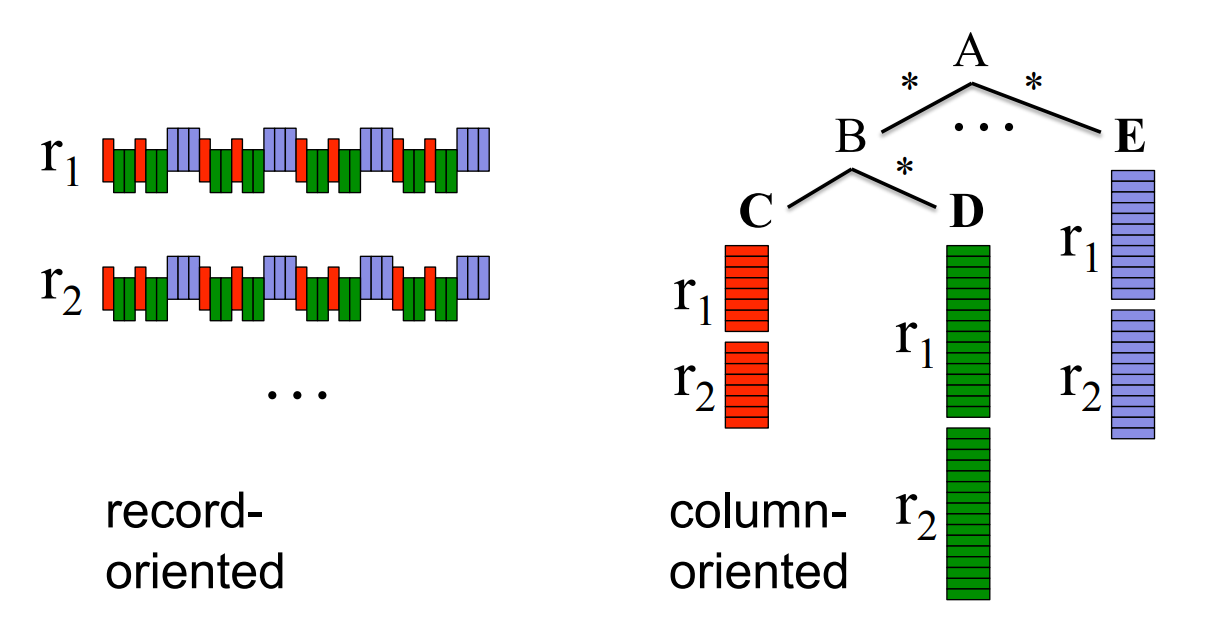
\includegraphics[width=0.95\linewidth]{google-dremel-fig1.png}
\end{center}

Source: \textcolor{blue}{\url{https://ai.google/research/pubs/pub36632}}
\end{frame}

\begin{frame}{On Scientific Linux, uproot/awkward is installed as often as Pandas}
\vspace{0.5 cm}
\begin{columns}
\column{1.2\linewidth}
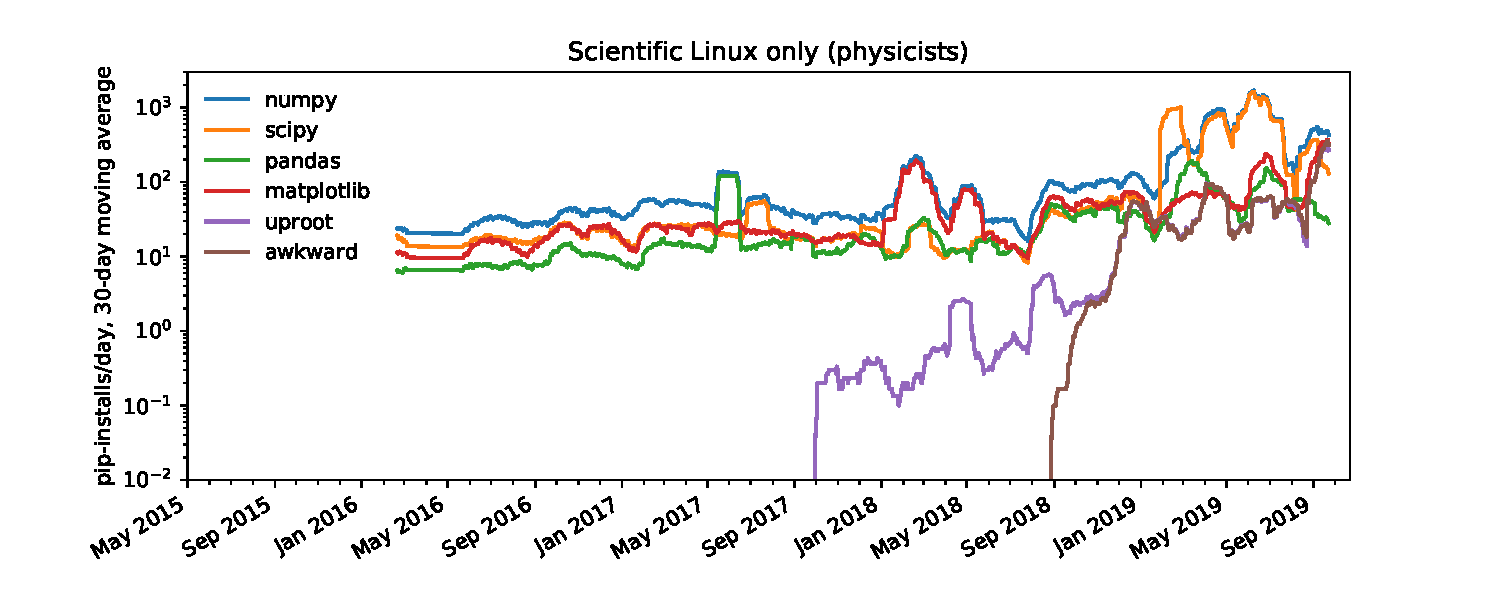
\includegraphics[width=\linewidth]{pip-scilinux-uproot.pdf}
\end{columns}
\end{frame}

\begin{frame}{And so is Coffea (very recently)\ldots}
\vspace{0.5 cm}
\begin{columns}
\column{1.2\linewidth}
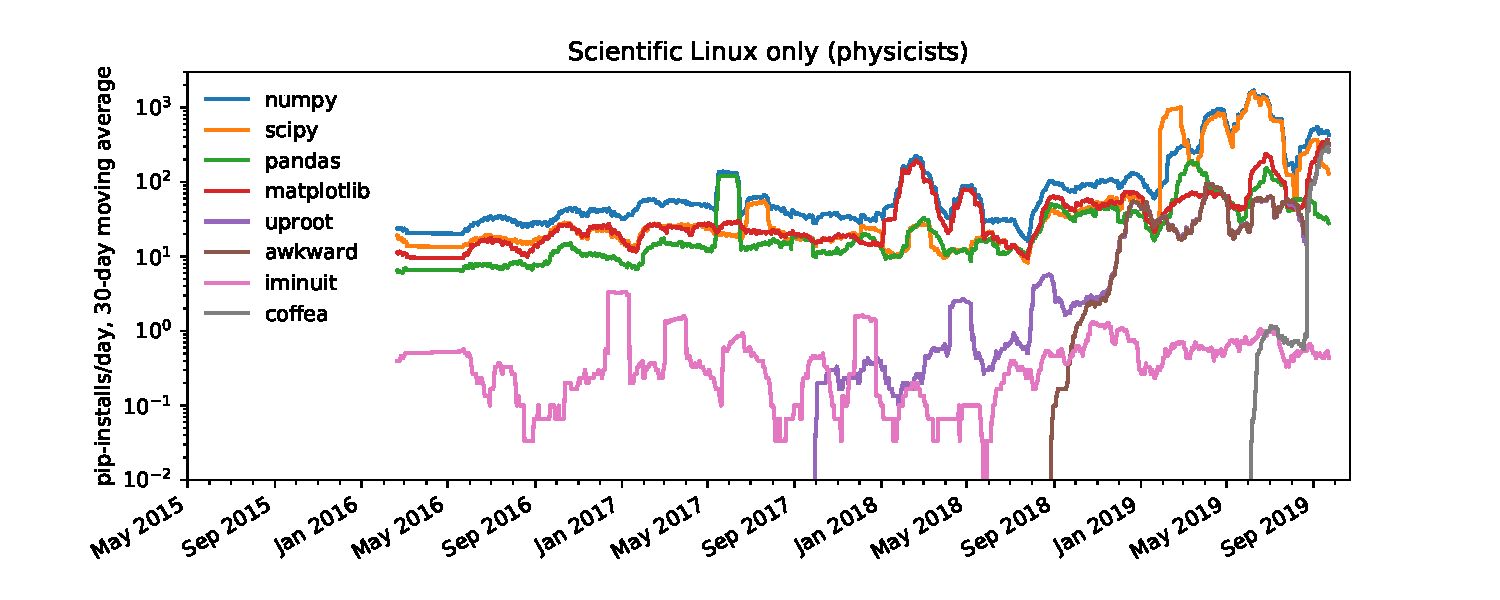
\includegraphics[width=\linewidth]{pip-scilinux-uproot-iminuit.pdf}
\end{columns}
\end{frame}

\begin{frame}{\ldots more so than deep learning libraries (TensorFlow and Torch)}
\vspace{0.5 cm}
\begin{columns}
\column{1.2\linewidth}
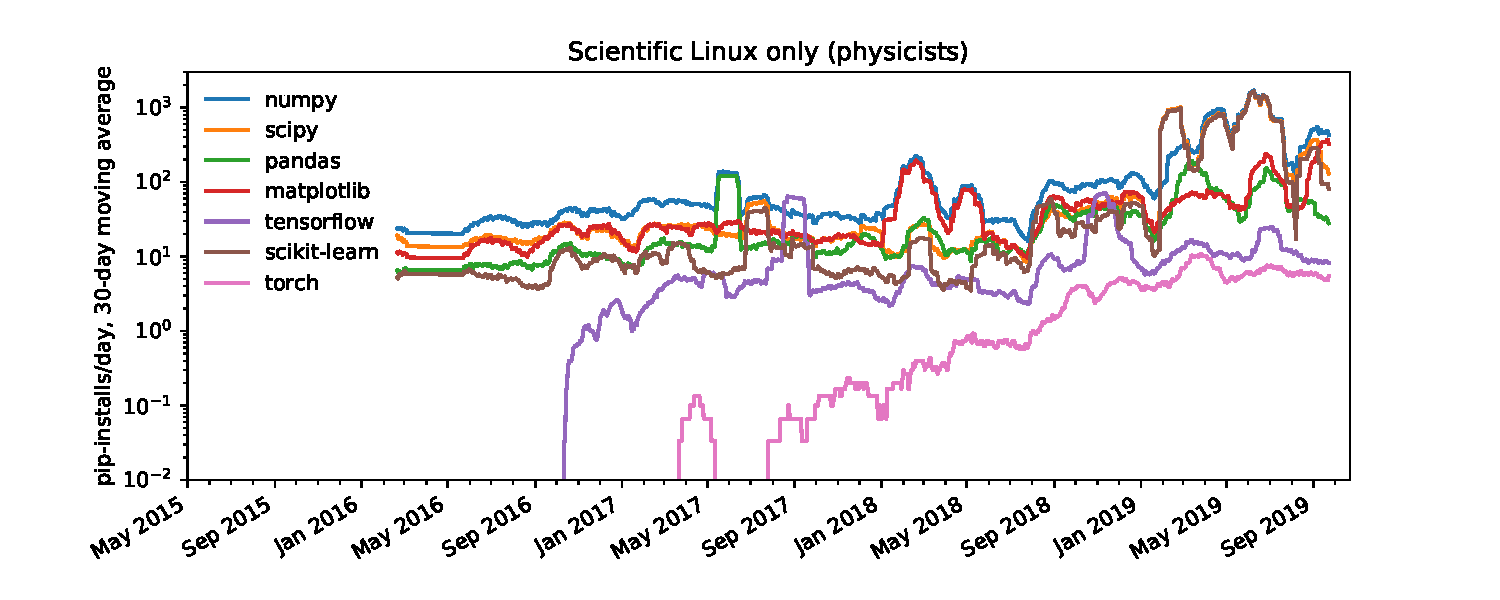
\includegraphics[width=\linewidth]{pip-scilinux-ml.pdf}
\end{columns}
\end{frame}

\begin{frame}{(Though in general, uproot is 4 orders of magnitude below Pandas)}
\vspace{0.5 cm}
\begin{columns}
\column{1.2\linewidth}
\only<1>{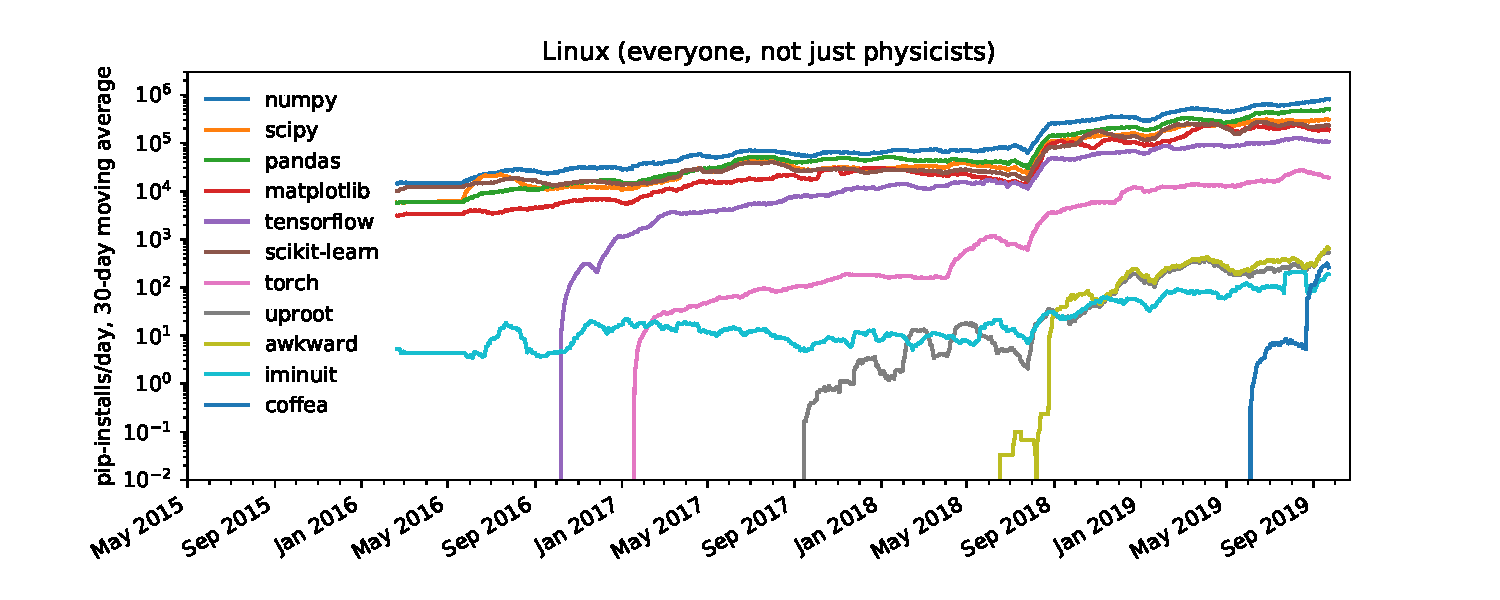
\includegraphics[width=\linewidth]{pip-linux.pdf}}\only<2>{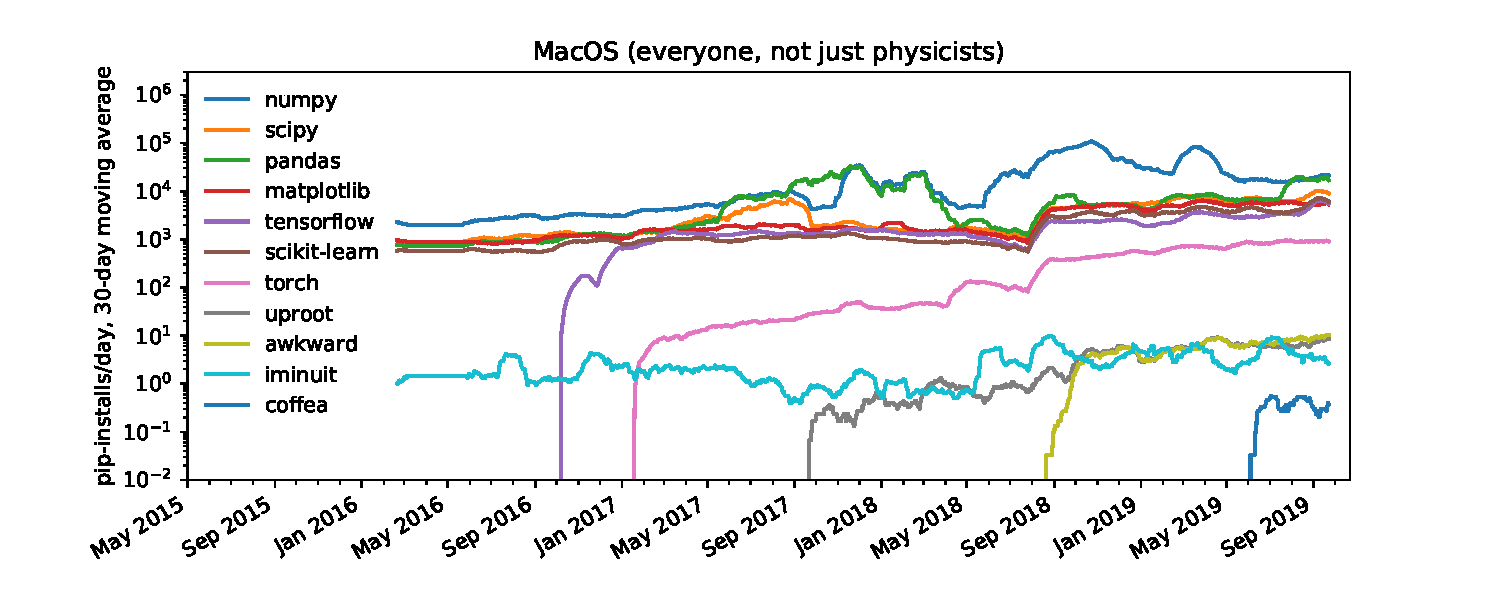
\includegraphics[width=\linewidth]{pip-macos.pdf}}\only<3>{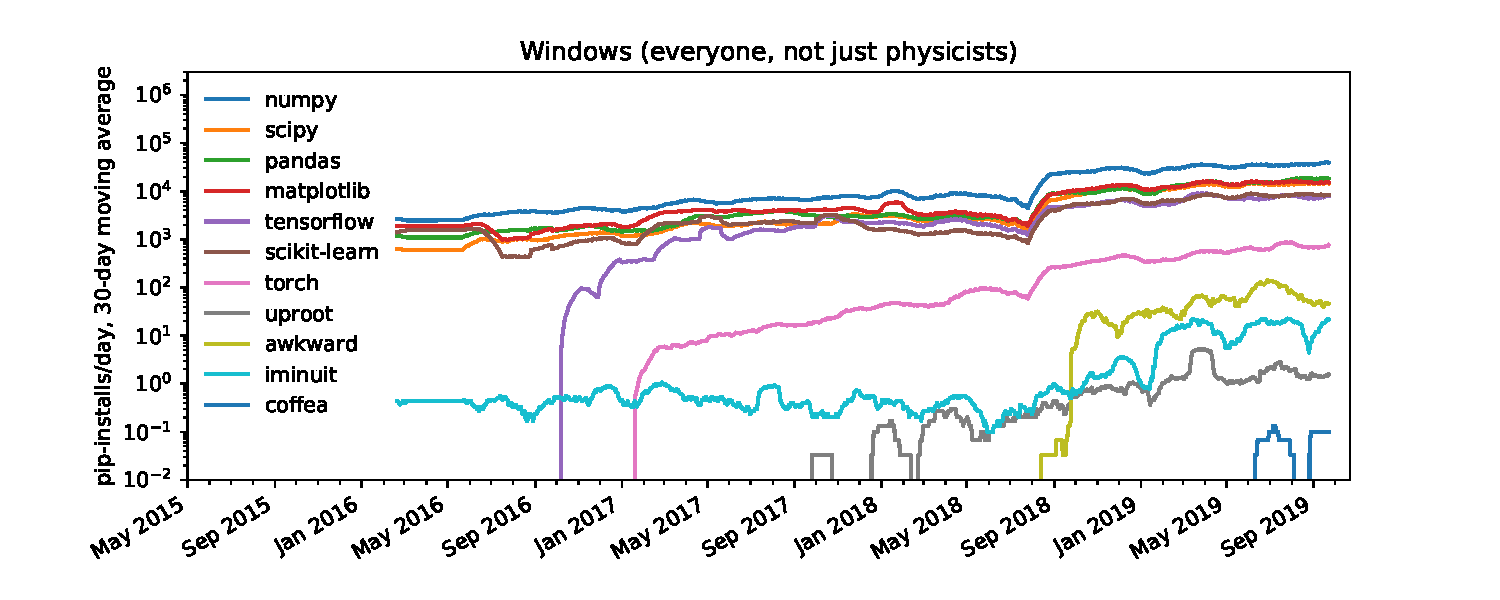
\includegraphics[width=\linewidth]{pip-windows.pdf}}
\end{columns}
\end{frame}

\begin{frame}{Uproot/Awkward maintainance is pretty much constant}
\Large
\vspace{0.75 cm}
\begin{columns}
\column{0.36\linewidth}
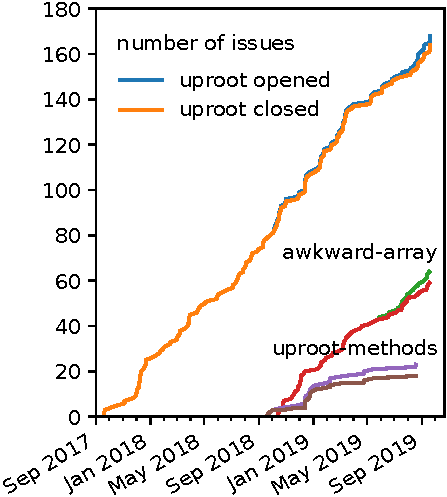
\includegraphics[width=\linewidth]{uproot-issues.pdf}

\column{0.72\linewidth}
\only<1>{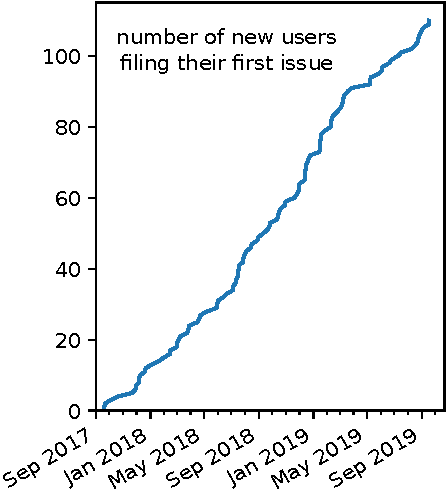
\includegraphics[width=0.5\linewidth]{uproot-users.pdf}\hfill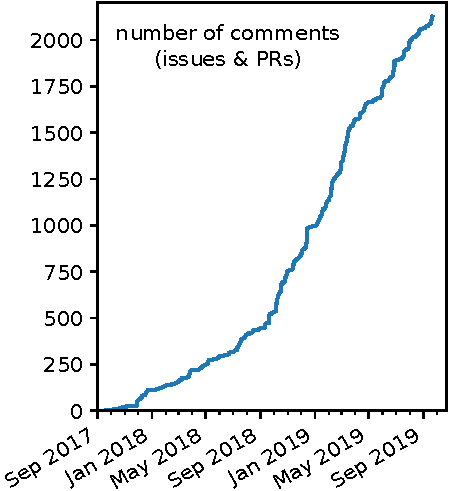
\includegraphics[width=0.5\linewidth]{uproot-comments.pdf}}\only<2->{\hfill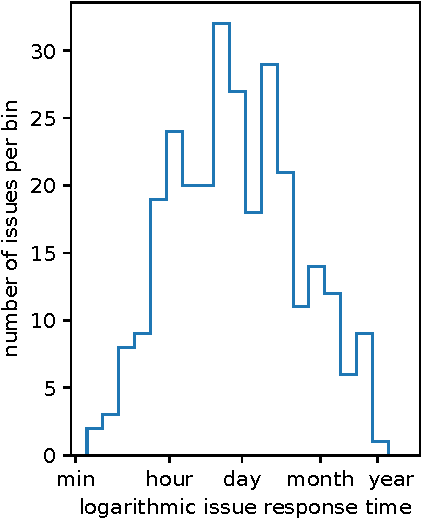
\includegraphics[width=0.45\linewidth]{uproot-response-time.pdf}\hfill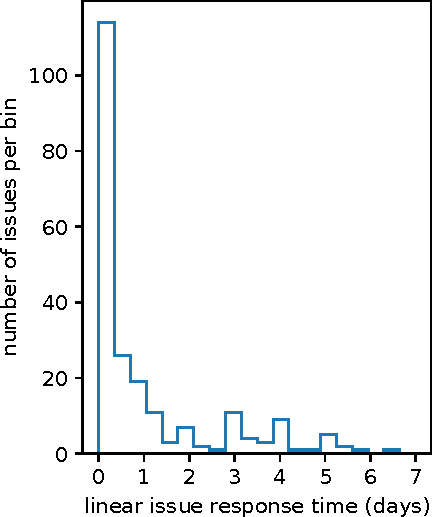
\includegraphics[width=0.45\linewidth]{uproot-response-time-linear.pdf}}
\end{columns}
\end{frame}

\begin{frame}{Awkward 1.0}
\large
\vspace{0.5 cm}
\begin{itemize}\setlength{\itemsep}{0.75 cm}
\item Uproot has been in use for 2 years now and is fine as-is. Maintenance with no major developments \textcolor{gray}{(apart from Pratyush's TTree-writing project)}.

\item Awkward has been in use for 1 year now, and there are

\vspace{0.2 cm}
\begin{itemize}\setlength{\itemsep}{0.2 cm}
\item structural issues: hard to keep interface consistent across all data types
\item interface issues: some visible features are confusing to users; need a semi-private between private and public.
\end{itemize}

\vspace{0.2 cm}
More detailed breakdown in this Google Doc (click): \normalsize

\vspace{0.2 cm}
\textcolor{blue}{\url{https://docs.google.com/document/d/1lj8ARTKV1_hqGTh0W_f01S6SsmpzZAXz9qqqWnEB3j4/edit?usp=sharing}}
\end{itemize}
\end{frame}

\begin{frame}{Awkward 1.0}
\vspace{0.2 cm}
\begin{columns}
\column{1.15\linewidth}
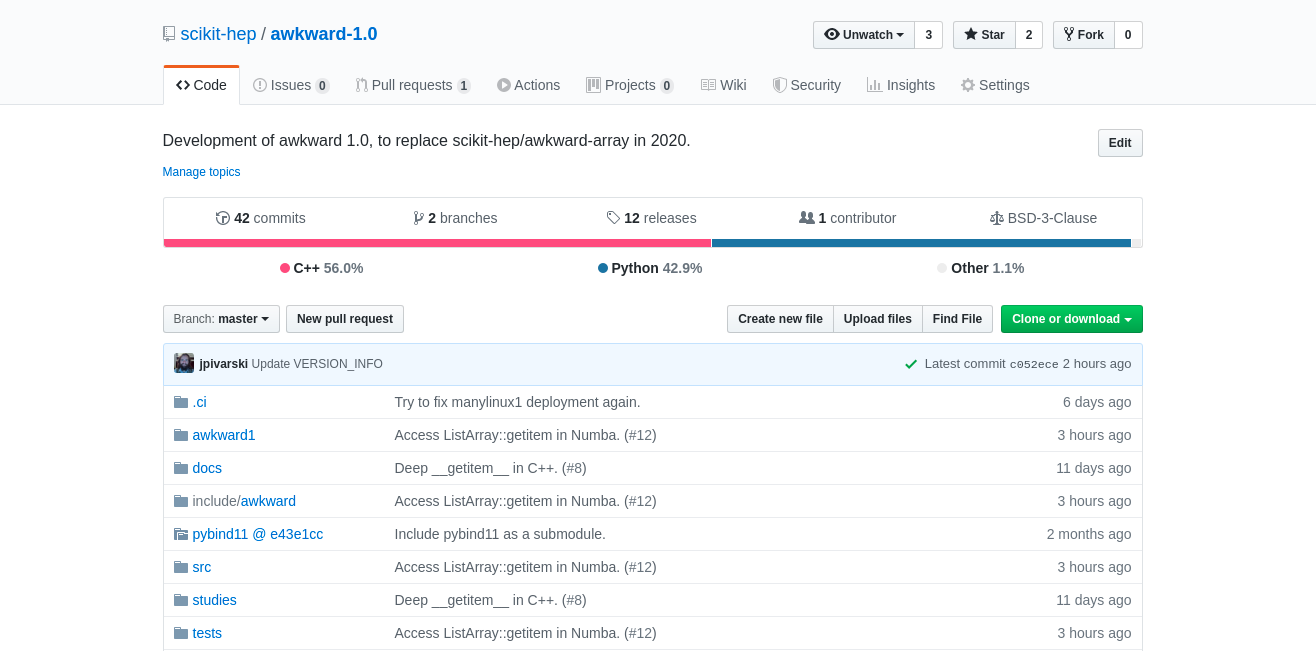
\includegraphics[width=\linewidth]{awkward-1-github.png}
\end{columns}
\end{frame}

\end{document}
